	\documentclass[10pt,oneside]{CBFT_book}
	% Algunos paquetes
	\usepackage{amssymb}
	\usepackage{amsmath}
	\usepackage{graphicx}
	\usepackage{libertine}
	\usepackage[bold-style=TeX]{unicode-math}
	\usepackage{lipsum}

	\usepackage{natbib}
	\setcitestyle{square}

	\usepackage{polyglossia}
	\setdefaultlanguage{spanish}


	\usepackage{CBFT.estilo} % Cargo la hoja de estilo

	% Tipografías
	% \setromanfont[Mapping=tex-text]{Linux Libertine O}
	% \setsansfont[Mapping=tex-text]{DejaVu Sans}
	% \setmonofont[Mapping=tex-text]{DejaVu Sans Mono}

	%===================================================================
	%	DOCUMENTO PROPIAMENTE DICHO
	%===================================================================

\begin{document}

% =================================================================================================
\chapter{Campos de cargas en movimiento}
% =================================================================================================

% =================================================================================================
\section{Potenciales retardados}
% =================================================================================================

Usando el gauge de Lorentz y las ecuaciones de Maxwell se llega a
\[
	\lapm{\vb{A}} - \frac{1}{c^2} \dpar[2]{\vb{A}}{t} = -\frac{4\pi}{c} \vb{J}
\]
\[
	\lapm{\phi} - \frac{1}{c^2} \dpar[2]{\phi}{t} = - 4 \pi \phi
\]
con forma general 
\be
	\lapm{\psi} - \frac{1}{c^2} \dpar[2]{\psi}{t} = - 4 \pi f(\vb{x},t)
	\label{onda_general}
\ee
siendo $f$ la que da la distribución de fuentes.

Resolveremos \eqref{onda_general} con una función de Green. Hacemos Fourier respecto a la frecuencia, de
manera que podamos remover el tiempo (además luego nos interesarán fuentes armónicas y por sobre todo
cualquier perturbación puede descomponerse en Fourier).

Suponemos que podemos escribir
\[
	\psi(\vb{x},t) = \frac{1}{2\pi}\int_{-\infty}^{+\infty} \psi(\vb{x},\omega) \euler^{-i\omega t} 
	d\omega
\]
\[
	f(\vb{x},t) = \frac{1}{2\pi}\int_{-\infty}^{+\infty} f(\vb{x},\omega) \euler^{-i\omega t} d\omega
\]
siendo sus inversas
\[
	\psi(\vb{x},\omega) = \int_{-\infty}^{+\infty} \psi(\vb{x}, t) \euler^{i\omega t} dt
\]
\[
	f(\vb{x},\omega) = \int_{-\infty}^{+\infty} f(\vb{x},t) \euler^{i\omega t} dt
\]
luego la ecuación resulta 
\[
	\int_{-\infty}^{+\infty} \lapm{\psi}(\vb{x},\omega) \euler^{ -i\omega t} d\omega +
	\int_{-\infty}^{+\infty} \frac{\omega^2}{c^2}\psi(\vb{x},\omega) \euler^{ -i\omega t} d\omega = 
		- 4 \pi \int_{-\infty}^{+\infty} f(\vb{x},\omega) \euler^{ -i\omega t} d\omega
\]
de manera que se satisface la ecuación de Helmholtz inhomogénea,
\[
	(\nabla^2 + k^2)\psi(\vb{x},\omega) = - 4\pi f(\vb{x},\omega),
\]
para cada valor de frecuencia $\omega$.

Una función de Green satisfacerá 
\[
	(\nabla^2 + k^2) G(\vb{x},\vb{x}') = - 4\pi \delta(\vb{x}-\vb{x}'),
\]
donde $\vb{x}-\vb{x}' = \vb{R}$ y la función de Green será simétricamente esférica pues pedimos la
no existencia de contornos, entonces llamando a aquella $G_k(R)$ se tiene 
\[
	\frac{1}{R}\dtot[2]{}{R}(RG_k) + k^2 G_k = - 4 \pi \delta (\vb{R})
\]
donde hemos usado el laplaciano en esféricas. Debemos distinguir dos casos, si $R=0$ entonces la
anterior resulta 
\[
	\lim_{kR \to 0} G_k(R) = \frac{1}{R}
\]
mientras que de ser cierto $R\neq 0$ en cambio
\[
	\dtot[2]{}{R}(RG_k) + k^2 (RG_k) = 0
\]
y entonces se propone como solución general 
\[
	G_k(R) = \frac{ A }{ R } \euler^{ i k R } + \frac{ B }{ R } \euler^{ -i k R }
\]
donde $A, B$ dependerán de las condiciones de contorno y siendo que el primer término del RHS representa
una onda divergente esférica y el segundo una onda convergente esférica.

Se puede interpretar $G_k$ como el potencial de una carga unitaria que aparece en $\vb{x}=\vb{x}'$ en el
instante $t=t'$ y luego desaparece (mmm, qué misterio!).

Ahora necesitamos meter la dependencia temporal,
\[
	\left(\nabla^2_x - \frac{1}{c^2}\dpar[2]{}{t} \right) G^{\pm}(\vb{x},\vb{x}',t,t') = 
	- 4 \pi \delta(\vb{x}-\vb{x}') \delta(t-t')
\]


\begin{figure}[htb]
	\begin{center}
	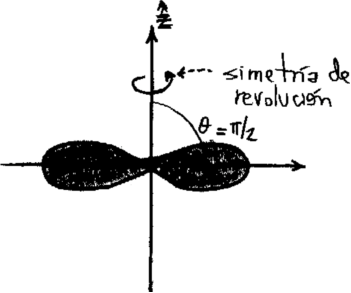
\includegraphics[width=0.4\textwidth]{images/fig_ft1_pot_irrad.pdf}	 
	\end{center}
	\caption{}
\end{figure} 

\begin{figure}[htb]
	\begin{center}
	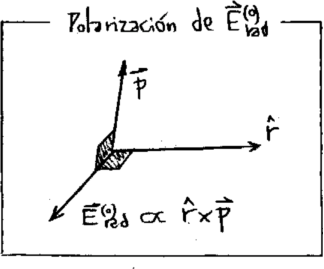
\includegraphics[width=0.4\textwidth]{images/fig_ft1_pot_irrad2.pdf}	 
	\end{center}
	\caption{}
\end{figure} 

\begin{figure}[htb]
	\begin{center}
	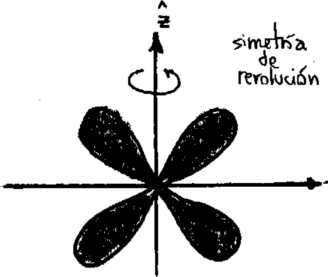
\includegraphics[width=0.4\textwidth]{images/fig_ft1_pot_irrad3.pdf}	 
	\end{center}
	\caption{}
\end{figure} 

% =================================================================================================
\section{Ejemplo de antena}
% =================================================================================================

\begin{figure}[htb]
	\begin{center}
	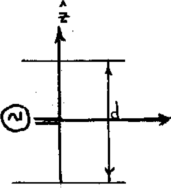
\includegraphics[width=0.4\textwidth]{images/fig_ft1_antena.pdf}	 
	\end{center}
	\caption{}
\end{figure} 

\begin{figure}[htb]
	\begin{center}
	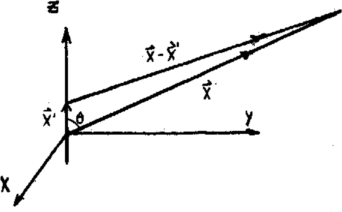
\includegraphics[width=0.4\textwidth]{images/fig_ft1_antena2.pdf}	 
	\end{center}
	\caption{}
\end{figure} 


\begin{figure}[htb]
	\begin{center}
	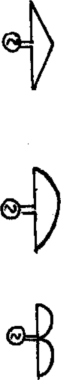
\includegraphics[width=0.4\textwidth]{images/fig_ft1_antena3.pdf}	 
	\end{center}
	\caption{}
\end{figure} 

% =================================================================================================
\section{Campos de una partícula cargada en movimiento}
% =================================================================================================

\begin{figure}[htb]
	\begin{center}
	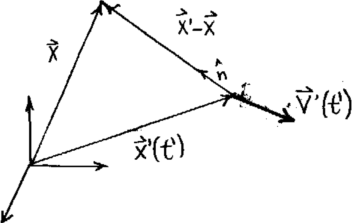
\includegraphics[width=0.4\textwidth]{images/fig_ft1_campo_part_car.pdf}	 
	\end{center}
	\caption{}
\end{figure} 

\begin{figure}[htb]
	\begin{center}
	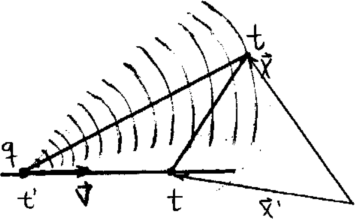
\includegraphics[width=0.4\textwidth]{images/fig_ft1_campo_part_car2.pdf}	 
	\end{center}
	\caption{}
\end{figure} 

% =================================================================================================
\section{Campo de una carga en movimiento}
% =================================================================================================

\begin{figure}[htb]
	\begin{center}
	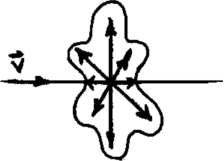
\includegraphics[width=0.4\textwidth]{images/fig_ft1_campo_carga_mov.pdf}	 
	\end{center}
	\caption{}
\end{figure} 

\begin{figure}[htb]
	\begin{center}
	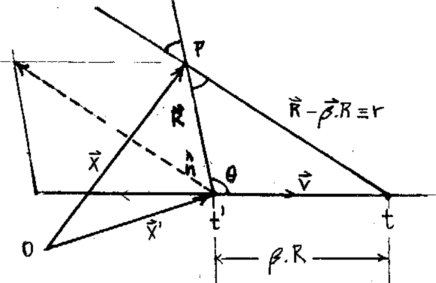
\includegraphics[width=0.4\textwidth]{images/fig_ft1_campo_carga_mov2.pdf}	 
	\end{center}
	\caption{}
\end{figure} 

% =================================================================================================
\section{Cálculo de potencia irradiada}
% =================================================================================================

\begin{figure}[htb]
	\begin{center}
	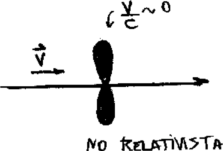
\includegraphics[width=0.4\textwidth]{images/fig_ft1_frenado2.pdf}	 
	\end{center}
	\caption{}
\end{figure} 

\begin{figure}[htb]
	\begin{center}
	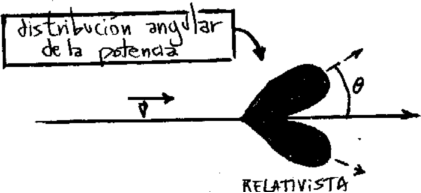
\includegraphics[width=0.4\textwidth]{images/fig_ft1_frenado3.pdf}	 
	\end{center}
	\caption{}
\end{figure} 

% =================================================================================================
\section{Frenado magnético}
% =================================================================================================

\begin{figure}[htb]
	\begin{center}
	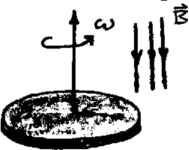
\includegraphics[width=0.4\textwidth]{images/fig_ft1_frenado.pdf}	 
	\end{center}
	\caption{}
\end{figure} 

% =================================================================================================
\subsection{Esponja electromagnética}
% =================================================================================================

\begin{figure}[htb]
	\begin{center}
	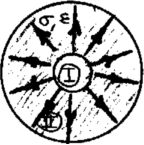
\includegraphics[width=0.4\textwidth]{images/fig_ft1_esponja.pdf}	 
	\end{center}
	\caption{}
\end{figure} 

% \bibliographystyle{CBFT-apa-good}	% (uses file "apa-good.bst")
% \bibliography{CBFT.Referencias} % La base de datos bibliográfica

\end{document}
